\problemname{Kitesurfing}

Nora the kitesurfer is taking part in a race across the Frisian islands, a very
long and thin archipelago in the north of the Netherlands.
The race takes place on the water and follows a straight line from start to finish.
Any islands on the route must be jumped over -- it is not allowed to surf around them.

The length of the race is $s$ metres and the archipelago consists of a number
of non-intersecting intervals between start and finish line.
During the race, Nora can move in two different ways:

\begin{enumerate}
  \item Nora can \emph{surf} between any two points at a speed of $1$ metre per
    second, provided there are no islands between them.
  \item Nora can \emph{jump} between any two points if they are at most $d$
    metres apart and neither of them is on an island. A jump always
    takes $t$ seconds, regardless of distance covered.
\end{enumerate}

While it is not possible to land on or surf across the islands,
it is still allowed to visit the end points of any island.

\vspace{-2mm}
\begin{figure}[!h]
  \centering
  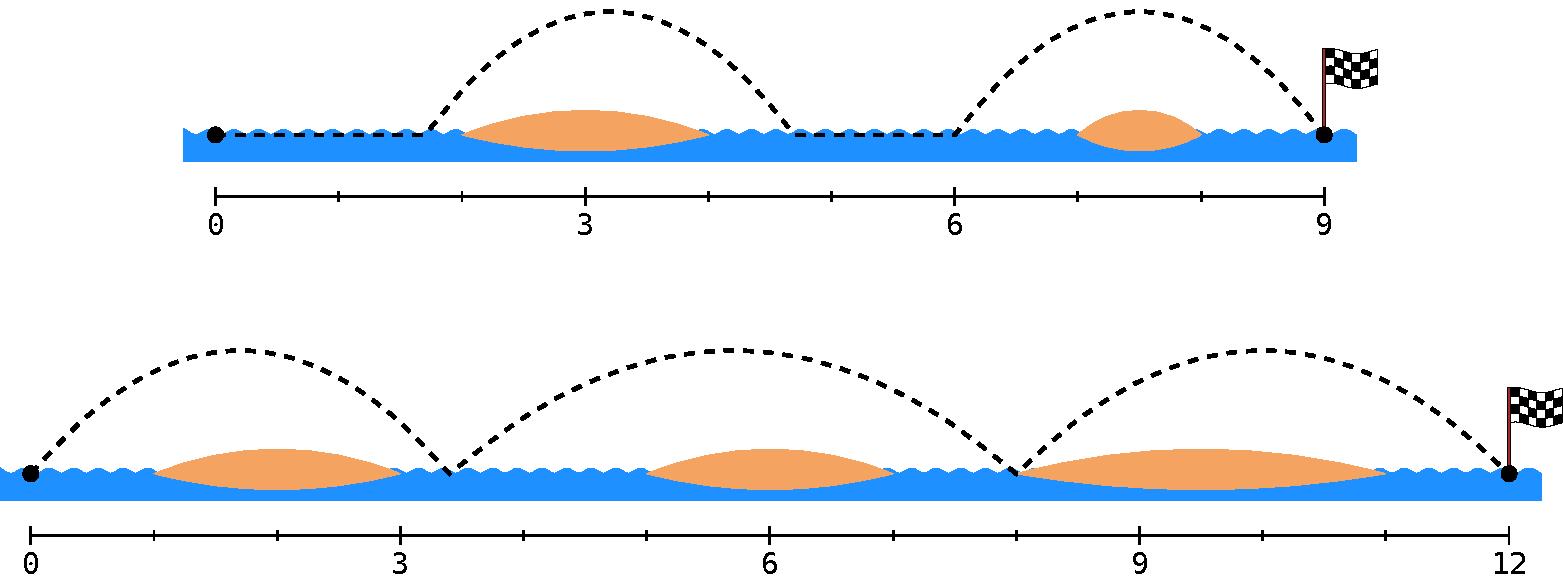
\includegraphics[width=0.8\textwidth]{samples}
  \caption{Illustration of the two sample cases.}
\end{figure}

Your task is to find the shortest possible time Nora can complete the race in.
You may assume that no island is more than $d$ metres long. In other words it is
always possible to finish the race.

\vspace{-2mm}
\section*{Input}

The input consists of:
\begin{itemize}
  \item One line with three integers $s,d$ and $t$ ($1 \le s,d,t \le 10^9$), where
    $s$ is the length of the race in metres,
    $d$ is the maximal jump distance in metres,
    and $t$ is the time needed for each jump in seconds.
  \item One line with an integer $n$ ($0 \le n \le 500$), the number of islands.
  \item $n$ lines, the $i$th of which contains two integers $\ell_i$ and $r_i$
    ($0 < \ell_i < r_i < s$ and $r_i-\ell_i \le d$), giving the boundaries of
    the $i$th island in metres, relative to the starting point.
\end{itemize}

The islands do not touch and are given from left to right,
that is $r_i < \ell_{i+1}$ for each valid $i$.

\vspace{-2mm}
\section*{Output}

Output one number, the shortest possible time in seconds needed to complete the race.
It can be shown that this number is always an integer.
